%
%
%

\begin{frame}[t]{Perceptron}

    The \index{perceptron}\Gls{perceptron} 
    is the simplest \index{neural network}neural network.

    It contains a single input layer and an output node.

    \begin{center}
        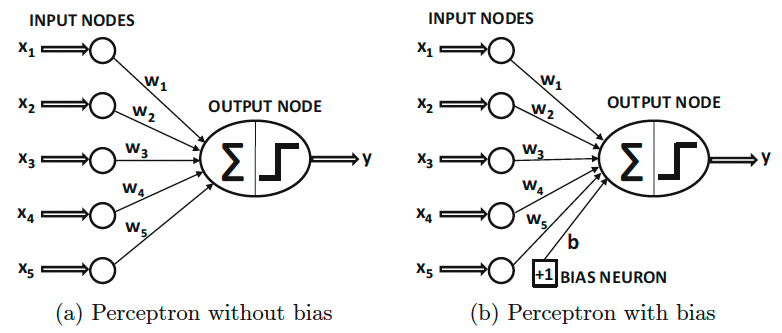
\includegraphics[width=0.85\textwidth]{./images/perceptron/basic_architecture.png}\\
        {\scriptsize \color{col:attribution} 
        Basic architecture of the perceptron. 
        Image reproduced from p.5 of \cite{Aggarwal:2018SpringerDL}}\\
    \end{center}

    It is a 
    \index{binary classification}binary classification 
    algorithm for 
    \index{supervised learning}supervised learning.

\end{frame}

%
%
%

\begin{frame}[t]{What problem does the perceptron tries to solve?}

    Consider the following problem. You have:
    \begin{itemize}
        \item a {\bf vector of $d$ feature variables}, $\vect{x}$ = $(x_1, x_2, ..., x_d)^T$, and
        \item a {\bf single binary variable} $y$ ($\in$ \{-1, +1\}).   
    \end{itemize}
    The binary variable $y$ \underline{depends on} the feature variables $\vect{x}$.\\
    \vspace{0.2cm}

    \begin{blockexample}{}
        \small
        For example:
        \begin{itemize}
            \small
            \item 
                $\vect{x}$: properties of a tumor imaged using computed tomography\\ 
                $y$: is the tumor is benign or malignant?
            \item 
                $\vect{x}$: features of an event observed in a particle physics detector\\ 
                $y$: is the event a new physics candidate 
                  or Standard Model background?
            \item 
                $\vect{x}$: details about a credit card transaction, such
                   as time, amount, location, and frequency of past transactions\\
                $y$: is the transaction fraudulent?
        \end{itemize}
    \end{blockexample}

\end{frame}

%
%
%

\begin{frame}[t]{What problem does the perceptron tries to solve?}

    Consider the following problem. You have:
    \begin{itemize}
        \item a {\bf vector of $d$ feature variables}, $\vect{x}$ = $(x_1, x_2, ..., x_d)^T$, and
        \item a {\bf single binary variable} $y$ ($\in$ \{-1, +1\}).   
    \end{itemize}
    The binary variable $y$ \underline{depends on} the feature variables $\vect{x}$.\\
    \vspace{0.4cm}
    We may have a \index{training set}{\bf training set} $\mathcal{D}$ that 
    consists of several ($\vect{x}$,$y$) examples.\\
    \begin{blockexample}{}
        \small
        For instance, we may have accumulated ($\vect{x}$,$y$) examples:
        \begin{itemize}
            \small
            \item from historical observations, or
            \item from simulations
        \end{itemize}
    \end{blockexample}  
    \vspace{0.2cm}
    Can we use the training set to {\bf learn the mapping} from $\vect{x}$ to $y$?\\
    \vspace{0.2cm}
    If we knew that mapping, we could apply it to new instances of $\vect{x}$
    for which $y$ is not known and needs to be predicted.
\end{frame}

%
%
%

\begin{frame}[t]{Perceptron}

    Let $\hat{y}$ be our prediction of $y$ for a given feature vector $\vect{x}$.
    The \index{perceptron}\gls{perceptron} computes the prediction as follows:
    \begin{equation}
        \hat{y} = sign\Big\{ \vect{w}^T \cdot \vect{x} \Big\} = sign\Big\{ \sum_{i=1}^{d} w_i x_i \Big\}
        \label{eq:perceptron_prediction_wo_bias}
    \end{equation}        

    \vspace{-1.0cm}

    \begin{columns}
        \begin{column}{0.50\textwidth}
         \begin{center}
          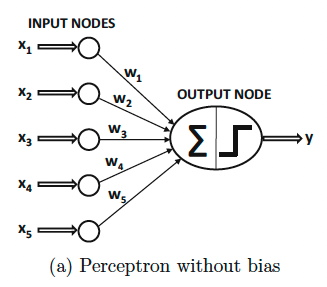
\includegraphics[width=0.95\textwidth]{./images/perceptron/perceptron_without_bias.png}\\
          {\scriptsize \color{col:attribution} 
          Image reproduced from p.5 of \cite{Aggarwal:2018SpringerDL}}\\
         \end{center}
        \end{column}
        \begin{column}{0.50\textwidth}
            \begin{itemize}
                \small
                \item Computes a linear function 
                ($\vect{w}^T \cdot \vect{x}$) in the output node.
                \item The sign function plays the role of
                an \index{activation function}\gls{activation function}.
                \item It maps a real value to either +1 or -1.
            \end{itemize}        
        \end{column}
    \end{columns}
      
\end{frame}

%
%
%

\begin{frame}[t]{Perceptron}

    We may need to add a \index{bias}{\bf bias} variable $b$, 
    to capture an invariant part of the prediction. 
    In this case, the \index{perceptron}\gls{perceptron} prediction is computed as follows:
    \begin{equation}
        \hat{y} = 
            sign\Big\{ \vect{w}^T \cdot \vect{x} + b \Big\} = 
            sign\Big\{ \sum_{i=1}^{d} w_i x_i + b \Big\}
            \label{eq:perceptron_prediction_w_bias}    
    \end{equation}

    \vspace{-1.0cm}

    \begin{columns}
        \begin{column}{0.50\textwidth}
         \begin{center}
            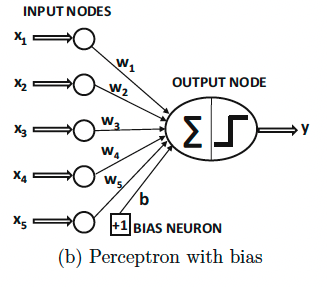
\includegraphics[width=0.95\textwidth]{./images/perceptron/perceptron_with_bias.png}\\
            {\scriptsize \color{col:attribution} 
            Image reproduced from p.5 of \cite{Aggarwal:2018SpringerDL}}\\
         \end{center}
        \end{column}
        \begin{column}{0.50\textwidth}
            \begin{itemize}
                \small
                \item Another approach to incorporate the bias, 
                is by \index{feature engineering}\gls{feature engineering}.
                \item Bias is the weight applied to an additional ($d$+1) 
                feature variable that always takes the value of 1.
                \item With that additional feature variable, 
                Eq. \ref{eq:perceptron_prediction_w_bias}
                can be reduced to Eq. \ref{eq:perceptron_prediction_wo_bias}.
                Therefore, for simplicity, will not show the bias explicitly.
            \end{itemize}        
        \end{column}
      \end{columns}

\end{frame}

%
%
%

\begin{frame}[t]{How does the perceptron learn?}

    The error of the prediction is:
    \begin{equation}
        E(\vect{x}) = y - \hat{y}
        \label{eq:perceptron_prediction_error}
    \end{equation}        
    where $\hat{y}$ is given by Eq. \ref{eq:perceptron_prediction_wo_bias} 
    (or Eq. \ref{eq:perceptron_prediction_w_bias})\\
    \vspace{0.5cm}

    $E(\vect{x})$ takes values from the set: \{ -2, 0, +2 \}.\\
    \begin{center}
        \begin{tabular}{rrcr}
            \hline
            $y$  & $\hat{y}$ & classification & $E(\vect{x})$ \\
            \hline
            -1   & -1  &   correct &   0  \\
            -1   & +1  &   wrong   &  -2  \\
            +1   & -1  &   wrong   &  +2  \\
            +1   & +1  &   correct &   0  \\
            \hline
    \end{tabular}
    \end{center}

    Similarly, to other \index{linear models}linear models in ML:
    If $E(\vect{x}) \ne 0$, the {\bf weights need to be updated in a 
    direction opposite to that of the error gradient}. 

\end{frame}

%
%
%

\begin{frame}[t]{The Mark 1 perceptron}

    The \index{perceptron}perceptron was invented in 1943 
    by W.\index{McCulloch}McCulloch and W.\index{Pitts}Pitts \cite{McCulloch:1943p}.
    \begin{itemize}
      \item It is sometimes called the \index{McCulloch-Pitts neuron}\gls{McCulloch-Pitts neuron}.
    \end{itemize}

    It was first implemented \underline{in hardware} in 1958, 
    by F.\index{Rosenblatt}\gls{Rosenblatt} \cite{Rosenblatt:1958p}.
    \begin{itemize}
        \item It is known as the \index{Mark 1 perceptron}\gls{Mark 1 perceptron}.
      \end{itemize}
  
    \begin{columns}[t]
        \begin{column}{0.25\textwidth}
         \begin{center}
            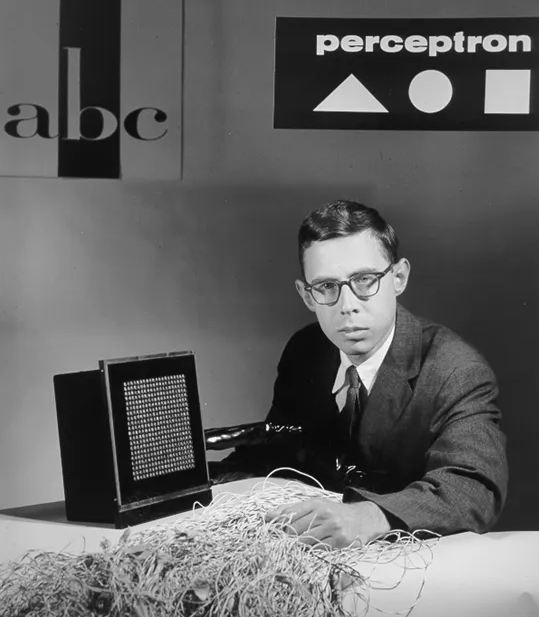
\includegraphics[width=0.95\textwidth]{./images/people/rosenblat_1.png}\\
            {\tiny 
            Rosenblatt and a part of his perceptron.\\
            \color{col:attribution} 
            Image reproduced from \cite{AIPlainEng:RiseAndFallOfPerceptron}\\}
         \end{center}
        \end{column}
        \begin{column}{0.50\textwidth}
            \begin{center}
                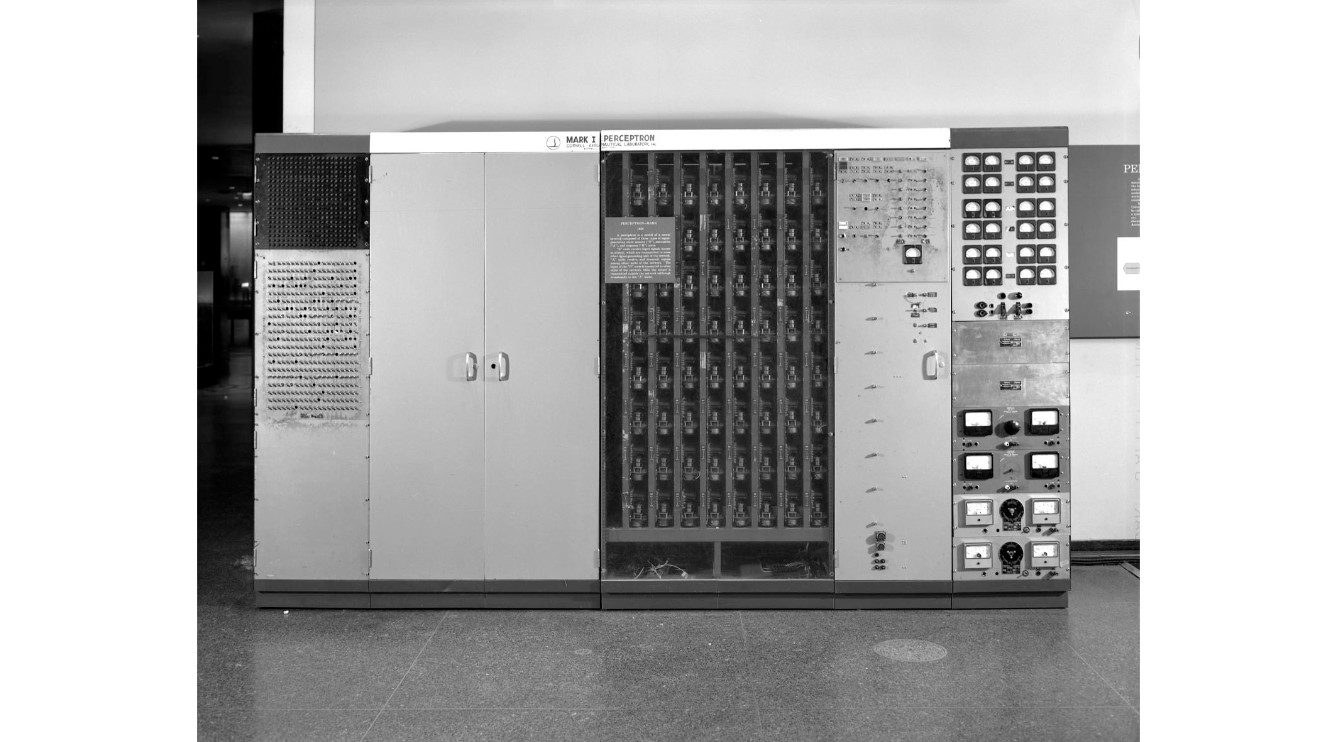
\includegraphics[width=0.98\textwidth]{./images/perceptron/mark1.png}\\
                {\tiny 
                The Mark 1 perceptron.\\
                \color{col:attribution} 
                Courtesy of The Smithsonian Institute\\ (Source: National Museum of American History)\\}
             \end{center}
        \end{column}
        \begin{column}{0.20\textwidth}
        \end{column}
      \end{columns}

\end{frame}

%
%
%

\begin{frame}[t]{Perceptron}

    \begin{equation}
        L = \sum_{(\vect{x},y) \in \mathcal{D}} (y - \hat{y})^2 
          = \sum_{(\vect{x},y) \in \mathcal{D}} \Bigg(y - sign\Big\{ \vect{w}^T \cdot \vect{x} \Big\}\Bigg)
     \end{equation}


\end{frame}

%
%
%

\begin{frame}[t]{Perceptron}

\end{frame}

%
%
%

\begin{frame}[t]{Perceptron}

\end{frame}
